% SOICT 2026 submission — Springer CCIS format (single-blind: keep author names).
% Requires the Springer LNCS/CCIS class `llncs.cls` + `splncs04.bst` from
% https://soict.org/wp-content/uploads/2025/09/Latex-Template-for-Springer.zip
% Max 12 pages excluding references. Figure: docs/paper/diagrams/soict_harlstmgat.{pdf,png}.
%
% VERSION 2026-09-05 v4 (= v3 + citation-review fixes + adversarial-review fixes).
%   Citation review (docs/paper/soict_harlstmgat_2026-09-04_citation_review_*.md) applied:
%   parkinson1980 at first use; karpoff1987 for volume-volatility motivation (predictive, not causal);
%   petersen2009 for cross-sectional-dependence inference (sqrt(N) qualified, not asserted as a rule);
%   bollerslev1986 for GARCH; patton2011 on QLIKE (asymmetry softened); "hard to beat"/"close to
%   optimal" softened to strong-benchmark/limited-room; spillover->cross-sectional dependence
%   (predictive, not causal); split-invariance narrowed to a multiplicative split factor; VN30>VN100
%   mean pairwise corr (0.345 vs 0.270) now computed + windowed in Data; clements2024/gnarharx2025
%   metadata completed (verified). Adversarial-review fixes: VN30 "best QLIKE at every horizon"->three
%   of four (LSTM edges h10); VN100 h10 graph favoured (was mislabelled LSTM); floor sourced from config.
% VERSION 2026-09-05 v3 (adds the contemporaneous-edge ablation to v2; structure per
% docs/paper/PAPER_LAYOUT_RULES.md). v3 = v2 verbatim + a new ablation subsection
% (Sec. Edge construction) and matching Discussion/Limitations notes. NOTHING in the
% delivered v2 tables/numbers is changed.
% Primary/headline market = VN100 (larger, more liquid; graph branch significant there).
% VN30 is a cross-market ablation. Pooled/transfer VN30 ablation is COMPLETE (all 4 horizons).
% NEW in v3: contemporaneous-correlation edge probe on VN100 AND VN30, uniform shorter
%   walk-forward (7 folds, 3 seeds, all horizons) reported HONESTLY as a probe, NOT as an
%   improvement over the directed volume->Parkinson edge. Prior mixed-protocol JSONs
%   (h10/h22 at 6f/5s) were discarded and re-run at 7f/3s for consistency.
% Estimator tables and HNX/HOSE/S&P 500 walk-forward remain [provisional] / % TODO.
% All numbers read from
%   results/walkforward_volga/walkforward_volga_{vn100,vn30}_h{1,5,10,22}.json (metrics[model].{mse,rmse,mae,qlike}, dm_date_clustered)
%   results/pooled_transfer_vn30/pooled_vn30_h{1,5,10,22}.json
%   results/contemp_edge/contemp_contemp_{vn100,vn30}_h{1,5,10,22}.json (metrics[model].{mse,rmse,mae,qlike}, dm_date_clustered)
% cross-checked against deliverables/2026-09-04_paper_pipeline_review/RESULTS_SUMMARY.md.
\documentclass[runningheads]{llncs}
\usepackage{graphicx}
\graphicspath{{diagrams/}}   % figure lives in docs/paper/diagrams/ (do NOT add ./ — collides with output pdf)
\usepackage{booktabs}
\usepackage{amsmath}
\usepackage{placeins}
\usepackage[T1]{fontenc}

\begin{document}

\title{VolGA: A Temporal Graph-Attention Model for Multi-Horizon Stock Volatility Forecasting in the Vietnamese Market}

\author{Author One\inst{1} \and Author Two\inst{1}}
\authorrunning{VolGA: Multi-Horizon Volatility Forecasting}
\institute{Affiliation, City, Country \\ \email{\{author1,author2\}@example.edu}}

\maketitle

\begin{abstract}
Forecasting daily stock-price volatility --- how much a stock's price is likely to swing on a given
day --- is a core input to risk management and option pricing: a risk manager sizing exposure or a
trader pricing an option needs to know not only where a price may go but how turbulent the path will
be.

We study \emph{VolGA} (Volatility Graph-Attention), a model that fuses a per-stock temporal branch
with a graph-attention branch, for multi-horizon volatility forecasting, using Vietnam's VN100 index
panel as the primary test market and the smaller VN30 panel, together with a same-feature no-graph
LSTM and the widening of the training universe, as ablation studies. All feature-based models share
the same five inputs and forecast a high--low range (Parkinson) measure of daily variance at one,
five, ten and twenty-two trading days ahead, against the linear HAR and an extended HAR (HAR-X) as
econometric benchmarks, evaluated with a leakage-free walk-forward protocol over twenty-two folds and
five seeds on MSE, RMSE, MAE and QLIKE, with a date-clustered Diebold--Mariano test that accounts for
the cross-sectional dependence of the panel. On VN100 the directed volume$\to$Parkinson graph adds a
significant QLIKE gain over the same-feature no-graph LSTM at the daily and weekly horizons
($h1$: $p=0.008$; $h5$: $p=0.011$), and VolGA attains the lowest point QLIKE at the daily horizon
($0.4916$); the hard-to-beat HAR-X keeps the best point QLIKE at the remaining horizons and no deep
model attains a significantly lower QLIKE than HAR-X at any horizon. On the smaller VN30 panel the
graph is not distinguishable from the no-graph LSTM at any horizon, even though VN30 has the higher
mean pairwise correlation. A same-market probe that replaces the directed volume$\to$Parkinson edge
with a contemporaneous-correlation edge, run under a shorter walk-forward, does not overturn this
reading: it does not improve the graph's marginal value over the no-graph LSTM on QLIKE and
significantly hurts at the monthly horizon, so the graph's contribution remains loss- and
horizon-dependent and is not made robust by changing the edge (Sec.~\ref{sec:edge}). The reading is
that the graph's marginal value tracks node breadth and liquidity rather than pairwise-correlation
magnitude, and that the verdict is loss-function dependent.
\keywords{Volatility forecasting \and HAR \and LSTM \and Graph Attention Network \and Diebold--Mariano.}
\end{abstract}

\section{Introduction}
Financial markets are volatile: prices swing, and the size of those swings --- an asset's
\emph{volatility} --- is the standard measure of its risk. Because volatility drives how options
are priced, how much capital a position ties up, and how risk is budgeted across a portfolio,
forecasting it accurately is a long-standing problem in financial econometrics~\cite{corsi2009}.
Volatility is not observed directly; it is estimated from prices, so any forecast is a forecast of
an estimate. We target the daily \emph{Parkinson estimator}~\cite{parkinson1980}, which gauges a day's
variance from its high--low price range and uses more of the day's information than a close-to-close
measure; our
forecasting target is therefore a variance (a squared quantity), not a standard deviation.

The dominant benchmark is the HAR model~\cite{corsi2009}: a plain linear regression that predicts
tomorrow's volatility from its own averages over the last day, the last week (about five trading
days), and the last month (about twenty-two), summarising volatility's long memory with a handful
of coefficients. HAR is deliberately simple yet provides a strong low-complexity
benchmark~\cite{corsi2009,audrino2025}, but it treats each stock on
its own and ignores that stocks in the same market move together, so a shock in one stock is never
allowed to inform a forecast for another.

Two model families are widely proposed to close that gap. Sequence models such as the
LSTM~\cite{lstm1997} learn non-linear patterns in a stock's own history, and graph neural networks
--- here a Graph Attention Network (GAT)~\cite{gat2018} --- capture \emph{cross-sectional dependence},
the same-day co-movement of turbulence across related stocks, by letting each stock draw on an
attention-weighted average of its most relevant peers; the graph is a predictive device, not an
identified economic spillover mechanism. Whether these additions improve
out-of-sample volatility forecasts is mixed in the literature, and reported gains are often
confounded by evaluation choices --- for example counting many co-moving stocks as independent
evidence, which overstates statistical significance.

This paper asks \emph{where}, if anywhere, deep and graph models improve on the linear HAR
benchmark in the Vietnamese market. We take the VN100 index panel --- the larger, more liquid of the
two panels we study --- as the primary test market and the smaller VN30 panel as a cross-market
ablation, and, holding the five inputs and the data design fixed, compare an extended HAR (HAR-X), a
no-graph LSTM, and VolGA under one leakage-free walk-forward protocol so the only difference is the
model. The headline finding is stated plainly: on the VN100 panel the directed
volume$\to$Parkinson graph adds a significant QLIKE gain over the same-feature no-graph LSTM at the
daily and weekly horizons ($h1$: $p=0.008$; $h5$: $p=0.011$), and VolGA attains the lowest point
QLIKE at the daily horizon; on the smaller VN30 panel the graph is indistinguishable from the
no-graph LSTM at every horizon --- even though VN30 has the higher mean pairwise correlation --- so
the graph's marginal value appears to track node breadth and liquidity rather than correlation
magnitude. Across both panels and all four horizons no deep model has a significantly lower QLIKE
than the HAR-X benchmark, which keeps the best point QLIKE at most horizons.

Our contributions are: (i) a multi-horizon Vietnamese-market benchmark that holds the feature set
and data design fixed across HAR, HAR-X, a no-graph LSTM and VolGA on the VN100 and VN30 panels, so
any measured difference is attributable to a single component; (ii) the finding that the graph
branch's contribution over the same-feature LSTM is significant on the larger, more liquid VN100
panel at the short horizons but null on VN30, while on the primary QLIKE loss no learned model
improves on the linear HAR-X benchmark at any horizon; and (iii) a panel-correct significance
protocol --- because co-moving stocks are not independent, we cluster the Diebold--Mariano test by
date; ignoring this cross-sectional dependence can substantially overstate a test's
precision~\cite{petersen2009}. Every reported number is taken from a stored results file, and we document
the data-quality limitations --- notably the unverified split adjustment of the Vietnamese prices and
the variance (not standard-deviation) target --- rather than presenting the data as uniformly clean.

\paragraph{Terminology (for readers outside finance).}
\emph{Volatility}: the size of a stock's price fluctuations, the standard proxy for its risk.
\emph{Parkinson estimator}: a day's variance measured from its high--low price range; our
forecasting target is this variance (squared units), not the standard deviation.
\emph{HAR}: a linear model predicting volatility from its own daily, weekly, and monthly averages.
\emph{HAR-X}: HAR augmented with exogenous regressors~\cite{corsi2009,clements2024}.
\emph{GARCH}: a classical time-series model that carries variance forward from recent return shocks~\cite{bollerslev1986}.
\emph{QLIKE}: a proxy-robust error measure for volatility forecasts that stays reliable when the
target is a noisy proxy; in the ratio-based implementation used here its asymmetric shape makes
forecast under- and over-shoots matter differently~\cite{patton2011}.
\emph{Diebold--Mariano (DM) test}: a test of whether one forecast is more accurate than another by
more than chance, computed from their day-by-day loss differences.
\emph{Graph Attention Network (GAT)}: a model in which stocks are nodes and edges carry influence;
each stock updates from an attention-weighted average of its neighbours, capturing cross-stock
\emph{spillover}.
\emph{Horizon} $h$: how many trading days ahead we forecast ($h\in\{1,5,10,22\}$, roughly a day,
week, fortnight, and month).

\section{Related Work}
\textbf{HAR and classical models.} HAR~\cite{corsi2009} approximates the long memory of realized
volatility with a daily/weekly/monthly cascade; recent work reports that rolling-window and
specification choices, rather than model class, often account for measured differences from
HAR~\cite{audrino2025}. The ``-X'' extension augments HAR with exogenous regressors; the low-frequency
OHLC HAR-X of Clements, Preve and Tee~\cite{clements2024} validates a range-based target, and
network-augmented HAR-X analogues have been proposed~\cite{gnarharx2025}. HARQ~\cite{harq2016}
exploits measurement error, and GARCH-family models remain standard conditional-variance benchmarks;
we did not run GARCH in the present walk-forward and report it only as a reference class.
\textbf{Deep and graph models.} LSTMs~\cite{lstm1997} are widely applied to financial series, and
graph neural networks model cross-asset spillovers, e.g.\ Graph Attention Networks~\cite{gat2018},
multivariate realized-volatility GNNs~\cite{chen2022} and spillover-aware GNN-HAR
hybrids~\cite{gnnhar2025}; reported effects vary across studies and data designs. Volatility spillover
measurement has a long econometric tradition~\cite{dy2012}. \textbf{Graph construction.} Our graph
uses a directed volume$\to$Parkinson relation (each node attends to its Top-5 volume-shock leaders,
edge-weighted, over two hops), motivated by the documented volume--volatility
association~\cite{karpoff1987} and used here as a predictive design choice rather than a causal claim;
we also probe an alternative
contemporaneous-correlation edge as an ablation (Sec.~\ref{sec:edge}). \textbf{Evaluation.}
Volatility is latent, so we use the proxy-robust QLIKE loss~\cite{patton2011} alongside MSE, with
significance by the Diebold--Mariano test~\cite{dm1995} and the Harvey--Leybourne--Newbold
small-sample correction~\cite{hln1997}.

\section{Method}
\textbf{Target and features.} The target is the Parkinson variance~\cite{parkinson1980} at day
$t{+}h$, a non-negative point forecast. The primary target is short-term, horizons $h\in\{1,5\}$
(one trading day and one trading week ahead); $h\in\{10,22\}$ (two weeks and roughly one trading
month) are an extended study. All three feature-based models (HAR-X, LSTM, VolGA) use the same five
node features per ticker at $t$: the daily Parkinson variance, its 5-day rolling mean (weekly), its
22-day rolling mean (monthly), a market Parkinson factor (the causal cross-sectional median of the
square-root Parkinson variance) and a 22-day volume z-score.

\textbf{Volatility estimators.} The primary target is the Parkinson variance; the estimator ablation
of Sec.~\ref{sec:est} also considers the Rogers--Satchell and windowed Yang--Zhang estimators. From
the daily open $O$, high $H$, low $L$ and close $C$ ($\ln$ is the natural logarithm), each is a daily
variance estimator: Parkinson uses only the high--low range, Rogers--Satchell is drift-independent,
and Yang--Zhang is windowed over $n{=}22$ days.
\begin{align*}
\sigma^2_{\mathrm{Park}} &= \tfrac{1}{4\ln 2}\,\ln(H/L)^2,\\
\sigma^2_{\mathrm{RS}} &= \ln(H/C)\ln(H/O)+\ln(L/C)\ln(L/O),\\
\sigma^2_{\mathrm{YZ}} &= \sigma^2_{o}+k\,\sigma^2_{c}+(1-k)\,\overline{\sigma^2_{\mathrm{RS}}},
\end{align*}
where for Yang--Zhang $\sigma^2_{o}$ and $\sigma^2_{c}$ are the $n$-day sample variances of the
overnight return $\ln(O_t/C_{t-1})$ and the open-to-close return $\ln(C_t/O_t)$,
$\overline{\sigma^2_{\mathrm{RS}}}$ is the rolling mean of the daily Rogers--Satchell term, and
$k=0.34/(1.34+(n{+}1)/(n{-}1))$~\cite{yangzhang2000,rogers1991}.

\textbf{Models.} \emph{HAR} (baseline): pooled OLS on the daily/weekly/monthly Parkinson cascade,
linear. \emph{HAR-X} (extended baseline~\cite{corsi2009,clements2024}): pooled OLS on the five
features (the HAR cascade augmented with a market Parkinson factor and a volume z-score), linear;
its disclosed deviations from the canonical HAR-X are a range-based Parkinson target and a direct
single-day $t{+}h$ target. \emph{LSTM}: a two-layer LSTM (hidden 64) over the lookback window of the
five features; a single pooled model is trained over all tickers, each standardized by its own scaler
fit on training rows only, with a linear output inverse-transformed for evaluation (dropout, weight
decay, gradient clipping, ReduceLROnPlateau, early stopping). \emph{VolGA} (Fig.~\ref{fig:arch}): the
LSTM branch plus a Graph Attention Network branch~\cite{gat2018} that reads the five node features at
$t$ and attends over a directed volume$\to$Parkinson Top-5, edge-weighted, two-hop graph estimated on
training rows only; the branches are concatenated into an MLP head. Comparing VolGA against the
same-feature no-graph LSTM isolates the graph's contribution.

\textbf{Masked panel.} Not every stock is listed on every date. Rather than keep only the dates on
which all stocks trade (which discards most of the data), we keep every trading date and mask out
stocks not yet listed, with a mask-aware loss that ignores the masked stocks, so every model is
trained and evaluated on the same panel.

\textbf{Protocol.} We use an expanding-window walk-forward evaluation of twenty-two folds with a fixed
retrain cadence (a new model is fit every $K$ folds; the configuration is recorded in every results
file so the runs are reproducible), a lookback window of twenty-two trading days, and five seeds
(batch size $32$; the seed set is fixed across models). For the learned models we report, for each
metric, the seed-level metric summarised as the ensemble point value with the \emph{per-seed standard
deviation} on QLIKE, so seed sensitivity is visible rather than hidden by a seed-averaged prediction.
We report MSE, RMSE, MAE and QLIKE with equal weight; predictions are floored at $10^{-2}$ times the
per-node training mean, applied identically to every model. Significance uses the
\emph{date-clustered} Diebold--Mariano test on the five-seed ensemble (mean) forecast: the
per-observation loss differential is collapsed to one value per calendar date before the statistic
(HLN correction, HAC lag $h{-}1$) is computed. This is the panel-correct treatment for a cross-section
that shares each trading date; a naive per-observation test treats the effective sample as the number
of tickers times the number of dates, which can substantially overstate precision when cross-sectional
dependence is ignored~\cite{petersen2009} --- under an independence approximation the overstatement
scales with about the square root of the number of stocks (of order ten on VN100, six on VN30), though
the exact factor depends on the panel's dependence structure. We report the targeted contrasts --- VolGA vs the
no-graph LSTM (the graph's marginal value) and VolGA vs HAR-X --- on QLIKE, squared error and
absolute error, because the verdict can be loss-dependent. Per-metric contrasts are reported without a
multiple-comparison correction (unadjusted).

\begin{figure}[t]
\centering
% figure generated by docs/paper/diagrams/generate_arch.py -> diagrams/soict_harlstmgat.{pdf,png,svg}
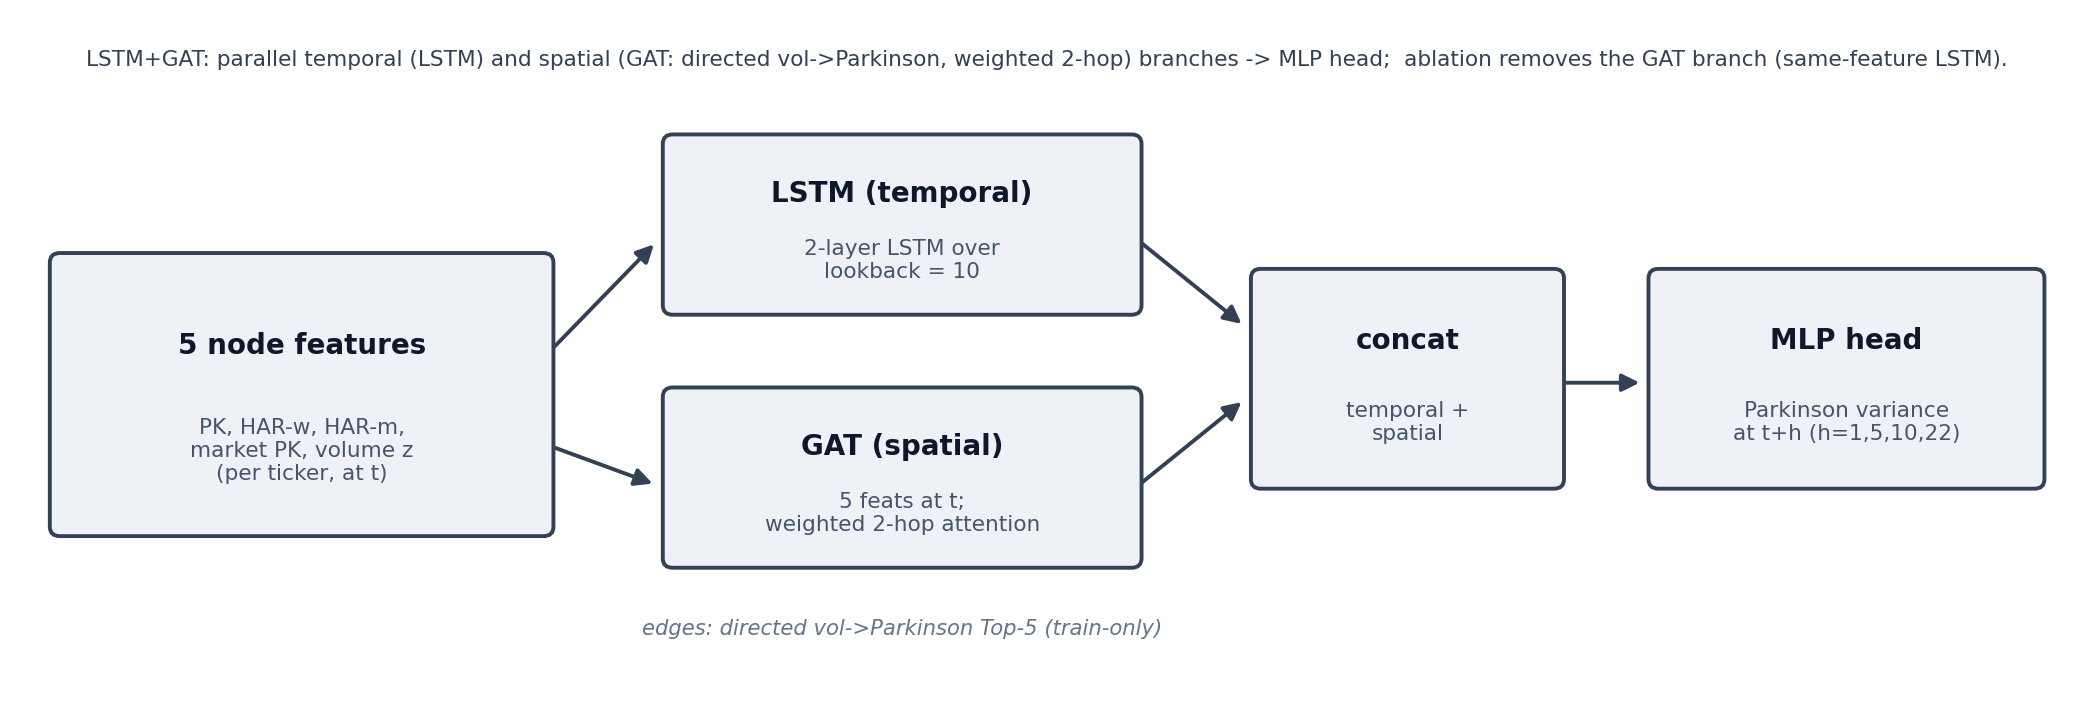
\includegraphics[width=\textwidth]{diagrams/soict_harlstmgat.png}
\caption{VolGA: a per-node LSTM temporal branch and a GAT spatial branch (directed volume$\to$Parkinson
Top-5 weighted two-hop attention) are concatenated into an MLP head; removing the GAT branch gives the
same-feature no-graph LSTM.}
\label{fig:arch}
\end{figure}

\section{Data}
The primary test market is the \textbf{VN100} index panel of the Vietnamese market (102 screened
tickers), the broader of the two panels; the \textbf{VN30} index panel (31 screened
tickers) serves as a cross-market ablation. Index membership follows the Ho Chi Minh Stock Exchange
index rules; both panels are additionally screened by trading history and liquidity, so ``broader''
refers to the larger, more actively traded VN100 constituent set. Both use the masked panel of Sec.~3
with the five features, per-ticker standardization fit on training rows only, and the walk-forward
protocol above. Over the full sample the mean pairwise correlation of the square-root Parkinson series
is higher on the smaller VN30 panel ($0.345$) than on VN100 ($0.270$), computed as the average
off-diagonal Pearson correlation across constituents. The main target is the Parkinson variance; the
windowed Yang--Zhang and Rogers--Satchell estimators appear in an ablation. The VN100 test sample is
46{,}308 masked observations over 454 out-of-sample dates at $h1$; the VN30 test sample is 10{,}881
masked observations over 351 out-of-sample dates at $h1$.

\section{Experiments}
The main comparison is the extended linear benchmark HAR-X and the proposed model VolGA (directed
volume$\to$Parkinson weighted two-hop) on the primary VN100 panel at horizons $\{1,5,10,22\}$,
reporting MSE, RMSE, MAE and QLIKE and the date-clustered Diebold--Mariano test (Table~\ref{tab:vn100main}).
The ablations then add the no-graph LSTM to isolate the graph branch on VN100 (Sec.~\ref{sec:graph}),
repeat the comparison on the smaller VN30 panel (Sec.~\ref{sec:vn30}), examine widening the deep
model's training universe (Sec.~\ref{sec:pool}), and probe an alternative graph edge --- a
contemporaneous-correlation edge in place of the directed volume$\to$Parkinson edge
(Sec.~\ref{sec:edge}); the alternative-estimator and additional-market studies (Sec.~\ref{sec:est})
are reported as far as the current runs allow.

\begin{table}[t]
\centering
\caption{Main result --- VN100 panel (102 nodes; 46{,}308 masked obs over 454 test dates at $h1$;
22 walk-forward folds, 5 seeds; VolGA: ensemble point value, QLIKE $\pm$~per-seed std). Lower is
better on every metric. MSE $\times10^{-7}$, RMSE/MAE $\times10^{-4}$.}
\label{tab:vn100main}
\footnotesize
\setlength{\tabcolsep}{6pt}
\begin{tabular}{llcccc}
\toprule
$h$ & Model & MSE & RMSE & MAE & QLIKE \\
\midrule
1 & HAR-X & 2.363 & 4.861 & 2.850 & 0.5004 \\
1 & VolGA & \textbf{2.348} & \textbf{4.846} & \textbf{2.816} & \textbf{0.4916}\,$\pm$.004 \\
\midrule
5 & HAR-X & \textbf{2.602} & \textbf{5.101} & 3.113 & \textbf{0.5610} \\
5 & VolGA & 2.615 & 5.114 & \textbf{3.067} & 0.5705\,$\pm$.013 \\
\midrule
10 & HAR-X & \textbf{2.748} & \textbf{5.242} & 3.247 & \textbf{0.6001} \\
10 & VolGA & 2.774 & 5.267 & \textbf{3.192} & 0.6149\,$\pm$.033 \\
\midrule
22 & HAR-X & \textbf{2.883} & \textbf{5.370} & 3.428 & \textbf{0.6388} \\
22 & VolGA & 2.913 & 5.397 & \textbf{3.352} & 0.6434\,$\pm$.003 \\
\bottomrule
\end{tabular}
\end{table}

\section{Results: the VN100 market}\label{sec:results}
On the primary VN100 panel (Table~\ref{tab:vn100main}) VolGA has the lowest point QLIKE at the daily
horizon ($h1$: $0.4916$ vs HAR-X $0.5004$) and the lowest MSE, RMSE and MAE there; at the weekly,
fortnightly and monthly horizons the linear HAR-X keeps the best point QLIKE, consistent with its
standing as a hard-to-beat benchmark. Across all four horizons VolGA has the lower MAE. The
date-clustered contrasts (Table~\ref{tab:dm-vn100}) show that no learned model attains a significantly
lower QLIKE than HAR-X at any horizon: the VolGA-vs-HAR-X QLIKE $p$-values are $0.177$, $0.585$,
$0.520$ and $0.842$. Where the deep models measurably differ from HAR-X is the absolute error, on
which VolGA is significantly lower at the short horizons ($h1$: $p<0.001$; $h5$: $p=0.005$; $h10$:
$p=0.032$). The proposed model therefore gives a significant point-error reduction on VN100 without a
significant QLIKE improvement over the linear benchmark.

\FloatBarrier
\section{Ablation studies}\label{sec:abl}
\subsection{Graph component (VN100)}\label{sec:graph}
Adding the no-graph LSTM to the primary comparison isolates the graph branch: removing the GAT branch
from VolGA gives the same-feature no-graph LSTM (Table~\ref{tab:vn100graph}), so the VolGA-vs-LSTM
contrast measures the graph's marginal value (Table~\ref{tab:dm-vn100}). On VN100 the graph adds a
significant QLIKE gain over the no-graph LSTM at the daily horizon ($h1$: $p=0.008$) and the weekly
horizon ($h5$: $p=0.011$); at $h10$ and $h22$ the graph-vs-LSTM QLIKE contrast is not significant
($p=0.229$ and $p=0.107$). Because the per-seed QLIKE standard deviation of the learned models is in
several cells of the same order as the graph-vs-LSTM difference, and the DM test is computed on the
five-seed ensemble forecast, the significant graph effect on VN100 is best read as an ensemble-level
regularity at the short horizons rather than a uniform per-seed gain.

\begin{table}[t]
\centering
\caption{Graph ablation --- VN100 panel: HAR-X, the no-graph LSTM, and the full VolGA (same scaling
and sample as Table~\ref{tab:vn100main}; learned models: ensemble point value, QLIKE $\pm$~per-seed
std). Lower is better on every metric.}
\label{tab:vn100graph}
\footnotesize
\setlength{\tabcolsep}{6pt}
\begin{tabular}{llcccc}
\toprule
$h$ & Model & MSE & RMSE & MAE & QLIKE \\
\midrule
1 & HAR-X & 2.363 & 4.861 & 2.850 & 0.5004 \\
1 & LSTM  & 2.355 & 4.853 & 2.821 & 0.5025\,$\pm$.020 \\
1 & VolGA & \textbf{2.348} & \textbf{4.846} & \textbf{2.816} & \textbf{0.4916}\,$\pm$.004 \\
\midrule
5 & HAR-X & \textbf{2.602} & \textbf{5.101} & 3.113 & \textbf{0.5610} \\
5 & LSTM  & 2.621 & 5.119 & 3.068 & 0.5763\,$\pm$.015 \\
5 & VolGA & 2.615 & 5.114 & \textbf{3.067} & 0.5705\,$\pm$.013 \\
\midrule
10 & HAR-X & \textbf{2.748} & \textbf{5.242} & 3.247 & \textbf{0.6001} \\
10 & LSTM  & 2.767 & 5.261 & \textbf{3.185} & 0.6096\,$\pm$.028 \\
10 & VolGA & 2.774 & 5.267 & 3.192 & 0.6149\,$\pm$.033 \\
\midrule
22 & HAR-X & \textbf{2.883} & \textbf{5.370} & 3.428 & \textbf{0.6388} \\
22 & LSTM  & 2.921 & 5.404 & 3.370 & 0.6479\,$\pm$.007 \\
22 & VolGA & 2.913 & 5.397 & \textbf{3.352} & 0.6434\,$\pm$.003 \\
\bottomrule
\end{tabular}
\end{table}

\begin{table}[t]
\centering
\caption{Date-clustered DM contrasts on VN100 ($p$-value; favoured model in parentheses; bold when
$p<0.05$; unadjusted). ``Graph'' is VolGA vs the same-feature no-graph LSTM on QLIKE (the graph's
marginal value); the remaining columns are VolGA vs HAR-X on QLIKE and on MAE.}
\label{tab:dm-vn100}
\footnotesize
\setlength{\tabcolsep}{6pt}
\begin{tabular}{lccc}
\toprule
$h$ & Graph (VolGA vs LSTM, QLIKE) & VolGA vs HAR-X (QLIKE) & VolGA vs HAR-X (MAE) \\
\midrule
1  & \textbf{0.008 (VolGA)} & 0.177 (VolGA) & \textbf{$<$0.001 (VolGA)} \\
5  & \textbf{0.011 (VolGA)} & 0.585 (HAR-X) & \textbf{0.005 (VolGA)} \\
10 & 0.229 (LSTM)           & 0.520 (HAR-X) & \textbf{0.032 (VolGA)} \\
22 & 0.107 (VolGA)          & 0.842 (HAR-X) & 0.094 (VolGA) \\
\bottomrule
\end{tabular}
\end{table}

\subsection{Other market: VN30}\label{sec:vn30}
Repeating the comparison on the smaller VN30 panel (Table~\ref{tab:vn30}) reverses the graph verdict.
The classical HAR (not shown; QLIKE $0.4952$ at $h1$) and HAR-X keep the best point QLIKE at most
horizons, and among the three models shown the linear HAR-X has the lowest QLIKE at $h1$, $h5$ and
$h22$. The date-clustered graph contrast (VolGA vs the no-graph LSTM on QLIKE) is not significant at
any horizon ($p=0.179$, $0.112$, $0.265$, $0.928$), and the VolGA-vs-HAR-X QLIKE contrast is likewise
not significant anywhere ($p=0.157$, $0.397$, $0.717$, $0.788$). VN30 carries the higher mean
pairwise correlation than VN100 yet shows the null graph effect, so the graph's marginal value appears
to scale with the number of nodes and their liquidity --- how many stable, informative edges the
attention can draw on --- rather than with correlation magnitude.

\begin{table}[t]
\centering
\caption{Market ablation --- VN30 panel (31 nodes; 10{,}881 masked obs over 351 test dates at $h1$;
22 folds, 5 seeds; learned models: ensemble point value, QLIKE $\pm$~per-seed std). Same scaling as
Table~\ref{tab:vn100main}. ``DM graph'' is the date-clustered VolGA-vs-LSTM QLIKE $p$-value (n.s.\ at
every horizon).}
\label{tab:vn30}
\footnotesize
\setlength{\tabcolsep}{6pt}
\begin{tabular}{llccccc}
\toprule
$h$ & Model & MSE & RMSE & MAE & QLIKE & DM graph \\
\midrule
1 & HAR-X & 1.938 & 4.402 & 2.402 & \textbf{0.4967} & \\
1 & LSTM  & 1.905 & 4.365 & 2.378 & 0.5219\,$\pm$.016 & 0.179 \\
1 & VolGA & \textbf{1.890} & \textbf{4.348} & \textbf{2.362} & 0.5146\,$\pm$.006 & (n.s.) \\
\midrule
5 & HAR-X & 2.156 & 4.644 & 2.614 & \textbf{0.5937} & \\
5 & LSTM  & \textbf{2.130} & \textbf{4.616} & \textbf{2.564} & 0.6327\,$\pm$.022 & 0.112 \\
5 & VolGA & 2.135 & 4.621 & 2.573 & 0.6150\,$\pm$.023 & (n.s.) \\
\midrule
10 & HAR-X & 2.363 & 4.861 & 2.771 & 0.6394 & \\
10 & LSTM  & \textbf{2.351} & \textbf{4.849} & 2.778 & \textbf{0.6336}\,$\pm$.004 & 0.265 \\
10 & VolGA & 2.358 & 4.856 & \textbf{2.758} & 0.6485\,$\pm$.098 & (n.s.) \\
\midrule
22 & HAR-X & \textbf{2.751} & \textbf{5.245} & 3.015 & \textbf{0.6987} & \\
22 & LSTM  & 2.823 & 5.313 & \textbf{3.010} & 0.7056\,$\pm$.005 & 0.928 \\
22 & VolGA & 2.829 & 5.319 & 3.011 & 0.7053\,$\pm$.004 & (n.s.) \\
\bottomrule
\end{tabular}
\end{table}

\subsection{Widening the training universe (VN30 $\to$ VN100)}\label{sec:pool}
To ask whether the VN30 QLIKE ceiling reflects a shortage of training stocks, we train the deep
models on a single VN100 panel under two arms --- one restricted to the 31 VN30 tickers (Arm~0),
one using all 102 VN100 tickers (Arm~1) --- and score both on the identical 31 VN30 out-of-sample
points, with the paired date-clustered DM comparing Arm~1 against Arm~0 (Table~\ref{tab:pool}).
Across horizons the widened universe does not significantly lower QLIKE on VN30 (VolGA: not
significant at any horizon; LSTM: significant only at $h{=}10$), but it significantly reduces the
absolute error at $h{=}1$ through $h{=}10$ for both deep models, an effect that fades by $h{=}22$.
The benefit of pooling is thus loss- and horizon-dependent: it lowers the average point error at
short-to-medium horizons without translating into a QLIKE gain, consistent with the QLIKE null on
the standalone panels. Only Arm~0 vs Arm~1 is a valid comparison here; Arm~0 is fit on the VN100
grid (with the VN100 market factor) and is not the standalone-VN30 setup of Table~\ref{tab:vn30},
so its numbers are not cross-comparable to that table.

\begin{table}[h]\centering
\caption{Widening the training universe: paired date-clustered DM $p$-values, Arm~1 (VN100-trained)
vs Arm~0 (VN30-trained), both scored on the 31 VN30 stocks over the identical out-of-sample points.
A star marks $p<0.05$ in favour of the wider universe (Arm~1).}\label{tab:pool}
\begin{tabular}{llcccc}
\toprule
Loss & Model & $h{=}1$ & $h{=}5$ & $h{=}10$ & $h{=}22$ \\
\midrule
QLIKE & LSTM & 0.136 & 0.081 & 0.033* & 0.252 \\
QLIKE & VolGA & 0.147 & 0.666 & 0.405 & 0.263 \\
Abs. error & LSTM & $<$0.001* & 0.006* & 0.008* & 0.558 \\
Abs. error & VolGA & $<$0.001* & $<$0.001* & 0.001* & 0.117 \\
\bottomrule
\end{tabular}
\end{table}

\subsection{Edge construction: contemporaneous correlation vs directed volume$\to$Parkinson}\label{sec:edge}
The graph in the main model wires each node to its Top-5 directed volume$\to$Parkinson leaders. To
ask whether a different edge changes the graph's contribution, we re-run VolGA on the same VN100
panel and the same five features with the directed edge replaced by a symmetric
contemporaneous-correlation edge (same-day co-movement of the range measure), keeping every other
choice fixed; because the no-graph LSTM does not use any edge, it is unchanged by construction and
serves as the reference for the graph's marginal value.

\textbf{This is a shorter-protocol probe, and cross-run level comparison is confounded.} The probe
runs a uniform 7-fold, 3-seed walk-forward across all four horizons on both panels, against the 22
folds and 5 seeds of the delivered vol$\to$Parkinson run (Tables~\ref{tab:vn100main}--\ref{tab:dm-vn100}).
The two runs differ in fold and seed count as well as in the edge, so numbers are only comparable
\emph{within} a single run; a level comparison of a contemp cell against a delivered vol$\to$Parkinson
cell mixes the edge with the protocol. The confound is demonstrable at $h1$: the edge- and
seed-independent HAR is essentially unchanged across the two runs (QLIKE $0.4985$ in the probe vs
$0.4983$ delivered), but the no-graph LSTM's ensemble QLIKE is markedly lower in the short probe
($0.4938$ vs $0.5025$ delivered) \emph{even though the LSTM does not use the edge}, so the lower probe
VolGA QLIKE ($0.4889$) is largely a protocol effect rather than an edge effect. The graph's marginal
value (VolGA vs the no-graph LSTM under the \emph{same} protocol) is therefore the interpretable
quantity, and it is read within each probe run.

\textbf{On the graph's marginal value the contemporaneous edge is not an improvement over
vol$\to$Parkinson.} On the VN100 graph-contribution contrast (VolGA vs the no-graph LSTM,
Table~\ref{tab:dm-edge}) the contemporaneous edge carries no QLIKE significance at any horizon: the
graph is favoured at $h1$ ($p=0.223$), $h5$ ($p=0.054$, at the margin) and $h10$ ($p=0.221$) and the
no-graph LSTM only at $h22$ ($p=0.849$), none significant, whereas the delivered vol$\to$Parkinson
edge is QLIKE-significant at the short horizons (Table~\ref{tab:dm-vn100}). On squared and absolute error the picture is
loss-dependent: at $h1$ the contemporaneous graph is favoured (SE $p=0.042$, AE $p=0.002$), while at
$h10$ and $h22$ the no-graph LSTM is favoured on absolute error ($p=0.014$ and $p=0.017$); squared
error is not significant beyond the daily horizon. The metric values are in
Table~\ref{tab:edgemetrics}; per-seed dispersion is not stored in the probe files, so QLIKE is
reported as the ensemble point value without a $\pm$ term.

\textbf{On VN30 the deep models do not improve on the linear baselines, and the graph adds nothing.}
On the smaller panel (Tables~\ref{tab:edgemetrics-vn30}, \ref{tab:dm-edge-vn30}) HAR/HAR-X hold the
best QLIKE at three of the four horizons (the no-graph LSTM edges narrowly ahead at $h10$, $0.6371$ vs
HAR-X $0.6385$, not significant), and the learned models are markedly worse in QLIKE at the short
horizons ($h1$ HAR-X $0.4967$ vs VolGA $0.5403$; VolGA vs HAR-X QLIKE $p=0.007$ favouring HAR-X). The
graph's
marginal value over the no-graph LSTM is not significant on QLIKE at any horizon ($p=0.139$--$0.792$);
the only significant graph-contrast cells are on absolute error ($h1$ $p=0.036$ favouring the no-graph
LSTM), so the graph does not help on the small market.

\textbf{Verdict.} Changing the edge from directed volume$\to$Parkinson to contemporaneous correlation
does not overturn the paper's overall reading: the graph's marginal value over the no-graph LSTM
remains loss- and horizon-dependent and does not robustly beat the no-graph LSTM on either panel, and
on VN30 the deep and graph models do not improve on the linear baselines. Isolating the edge effect
cleanly requires a matched-protocol (same folds and seeds) vol$\to$Parkinson run; that run is future
work.

\begin{table}[t]
\centering
\caption{Contemporaneous-edge probe --- VN100 panel, HAR / HAR-X / no-graph LSTM / VolGA (contemp
edge). Uniform shorter walk-forward across horizons (7 folds, 3 seeds), against the 22 folds and 5
seeds of the delivered vol$\to$Parkinson run (Table~\ref{tab:vn100main}); learned models are ensemble
point values (per-seed dispersion not stored in the probe files). MSE $\times10^{-7}$, RMSE/MAE
$\times10^{-4}$. Lower is better on every metric. Not level-comparable to Table~\ref{tab:vn100main}
(different protocol).}
\label{tab:edgemetrics}
\footnotesize
\setlength{\tabcolsep}{6pt}
\begin{tabular}{llcccc}
\toprule
$h$ & Model & MSE & RMSE & MAE & QLIKE \\
\midrule
1 & HAR   & 2.369 & 4.868 & 2.907 & 0.4985 \\
1 & HAR-X & 2.363 & 4.862 & 2.850 & 0.5006 \\
1 & LSTM  & 2.345 & 4.843 & 2.811 & 0.4938 \\
1 & VolGA & \textbf{2.331} & \textbf{4.828} & \textbf{2.793} & \textbf{0.4889} \\
\midrule
5 & HAR   & 2.625 & 5.124 & 3.152 & 0.5672 \\
5 & HAR-X & 2.603 & 5.102 & 3.114 & 0.5611 \\
5 & LSTM  & 2.604 & 5.103 & \textbf{3.064} & 0.5647 \\
5 & VolGA & \textbf{2.599} & \textbf{5.098} & 3.073 & \textbf{0.5606} \\
\midrule
10 & HAR   & 2.752 & 5.246 & 3.269 & 0.6003 \\
10 & HAR-X & \textbf{2.747} & \textbf{5.242} & 3.248 & \textbf{0.6000} \\
10 & LSTM  & 2.772 & 5.265 & \textbf{3.196} & 0.6147 \\
10 & VolGA & 2.774 & 5.267 & 3.221 & 0.6080 \\
\midrule
22 & HAR   & 2.885 & 5.371 & 3.425 & 0.6390 \\
22 & HAR-X & \textbf{2.883} & \textbf{5.369} & 3.429 & \textbf{0.6386} \\
22 & LSTM  & 2.935 & 5.418 & \textbf{3.385} & 0.6518 \\
22 & VolGA & 2.951 & 5.433 & 3.419 & 0.6527 \\
\bottomrule
\end{tabular}
\end{table}

\begin{table}[t]
\centering
\caption{Contemporaneous-edge probe --- VN30 panel (31 nodes), HAR / HAR-X / no-graph LSTM / VolGA
(contemp edge). Same protocol as Table~\ref{tab:edgemetrics} (7 folds, 3 seeds). MSE $\times10^{-7}$,
RMSE/MAE $\times10^{-4}$. Lower is better on every metric.}
\label{tab:edgemetrics-vn30}
\footnotesize
\setlength{\tabcolsep}{6pt}
\begin{tabular}{llcccc}
\toprule
$h$ & Model & MSE & RMSE & MAE & QLIKE \\
\midrule
1 & HAR   & 1.947 & 4.413 & 2.432 & \textbf{0.4954} \\
1 & HAR-X & 1.938 & 4.402 & 2.403 & 0.4967 \\
1 & LSTM  & 1.897 & 4.355 & \textbf{2.362} & 0.5475 \\
1 & VolGA & \textbf{1.891} & \textbf{4.348} & 2.373 & 0.5403 \\
\midrule
5 & HAR   & 2.171 & 4.659 & 2.636 & 0.5938 \\
5 & HAR-X & 2.156 & 4.643 & 2.613 & \textbf{0.5929} \\
5 & LSTM  & 2.142 & 4.628 & \textbf{2.586} & 0.6319 \\
5 & VolGA & \textbf{2.138} & \textbf{4.624} & 2.603 & 0.6272 \\
\midrule
10 & HAR   & 2.367 & 4.865 & 2.783 & 0.6405 \\
10 & HAR-X & 2.362 & 4.860 & \textbf{2.769} & 0.6385 \\
10 & LSTM  & \textbf{2.348} & \textbf{4.846} & 2.772 & \textbf{0.6371} \\
10 & VolGA & 2.353 & 4.851 & 2.770 & 0.6376 \\
\midrule
22 & HAR   & 2.755 & 5.248 & 3.016 & 0.7001 \\
22 & HAR-X & \textbf{2.749} & \textbf{5.243} & 3.015 & \textbf{0.6976} \\
22 & LSTM  & 2.836 & 5.326 & 3.024 & 0.7121 \\
22 & VolGA & 2.855 & 5.343 & \textbf{3.014} & 0.7188 \\
\bottomrule
\end{tabular}
\end{table}

\begin{table}[t]
\centering
\caption{Contemporaneous-edge probe --- date-clustered DM contrasts on VN100 ($p$-value; favoured
model in parentheses; bold when $p<0.05$; unadjusted). ``Graph'' is VolGA (contemp edge) vs the
same-feature no-graph LSTM (the graph's marginal value); the remaining block is VolGA vs HAR-X. Each
contrast is reported on QLIKE, squared error (SE) and absolute error (AE). Same protocol as
Table~\ref{tab:edgemetrics} (7 folds, 3 seeds).}
\label{tab:dm-edge}
\footnotesize
\setlength{\tabcolsep}{5pt}
\resizebox{\textwidth}{!}{%
\begin{tabular}{lcccccc}
\toprule
 & \multicolumn{3}{c}{Graph (VolGA vs LSTM)} & \multicolumn{3}{c}{VolGA vs HAR-X} \\
\cmidrule(lr){2-4}\cmidrule(lr){5-7}
$h$ & QLIKE & SE & AE & QLIKE & SE & AE \\
\midrule
1  & 0.223 (VolGA) & \textbf{0.042 (VolGA)} & \textbf{0.002 (VolGA)} & 0.061 (VolGA) & \textbf{0.022 (VolGA)} & \textbf{$<$0.001 (VolGA)} \\
5  & 0.054 (VolGA) & 0.394 (VolGA)          & 0.129 (LSTM)          & 0.971 (VolGA) & 0.820 (VolGA)          & \textbf{0.015 (VolGA)} \\
10 & 0.221 (VolGA) & 0.767 (LSTM)           & \textbf{0.014 (LSTM)} & 0.639 (HAR-X) & 0.192 (HAR-X)          & 0.357 (VolGA) \\
22 & 0.849 (LSTM)  & 0.076 (LSTM)           & \textbf{0.017 (LSTM)} & 0.492 (HAR-X) & \textbf{0.044 (HAR-X)} & 0.811 (VolGA) \\
\bottomrule
\end{tabular}}
\end{table}

\begin{table}[t]
\centering
\caption{Contemporaneous-edge probe --- date-clustered DM contrasts on VN30 ($p$-value; favoured
model in parentheses; bold when $p<0.05$; unadjusted). Blocks and metrics as in
Table~\ref{tab:dm-edge}; same protocol (7 folds, 3 seeds).}
\label{tab:dm-edge-vn30}
\footnotesize
\setlength{\tabcolsep}{5pt}
\resizebox{\textwidth}{!}{%
\begin{tabular}{lcccccc}
\toprule
 & \multicolumn{3}{c}{Graph (VolGA vs LSTM)} & \multicolumn{3}{c}{VolGA vs HAR-X} \\
\cmidrule(lr){2-4}\cmidrule(lr){5-7}
$h$ & QLIKE & SE & AE & QLIKE & SE & AE \\
\midrule
1  & 0.139 (VolGA) & 0.301 (VolGA) & \textbf{0.036 (LSTM)} & \textbf{0.007 (HAR-X)} & 0.083 (VolGA) & \textbf{0.028 (VolGA)} \\
5  & 0.659 (VolGA) & 0.644 (VolGA) & 0.053 (LSTM)          & 0.383 (HAR-X) & 0.352 (VolGA) & 0.507 (VolGA) \\
10 & 0.792 (LSTM)  & 0.176 (LSTM)  & 0.698 (VolGA)         & 0.951 (VolGA) & 0.540 (VolGA) & 0.966 (HAR-X) \\
22 & 0.252 (LSTM)  & 0.146 (LSTM)  & 0.559 (VolGA)         & 0.437 (HAR-X) & \textbf{0.041 (HAR-X)} & 0.975 (VolGA) \\
\bottomrule
\end{tabular}}
\end{table}

\subsection{Alternative volatility estimators}\label{sec:est}
\textbf{[provisional --- full estimator tables pending.]} The Parkinson variance is the chosen
range-based target for this market: prior investigation of the Rogers--Satchell, windowed
Yang--Zhang and close-to-close targets found worse forecast QLIKE, with the loss coming from
non-persistent overnight components that on the unadjusted Vietnamese prices carry corporate-action
jumps; the intraday high--low Parkinson estimator is invariant to price splits and is therefore
preferred. The multi-market, multi-estimator walk-forward tables (Rogers--Satchell and windowed
Yang--Zhang targets across markets) are not yet regenerated on the clean data and are omitted rather
than carried over from earlier runs.
% TODO(coordinator): regenerate estimator tables on clean-data walk-forward before submission.

\subsection{Additional markets}
\textbf{[provisional --- pending clean-data walk-forward.]} Extending the same protocol to the HNX and
HOSE exchanges and the U.S. S\&P 500 as a cross-market comparison is planned; those walk-forward runs
are not yet complete on the current clean data and are intentionally not reported here to avoid
presenting stale numbers as final.
% TODO(coordinator): add HNX / HOSE / S&P 500 clean-data walk-forward when available.

\FloatBarrier
\section{Discussion}\label{sec:disc}
\textbf{Graph contribution.} The directed volume$\to$Parkinson graph adds a significant QLIKE gain
over the same-feature no-graph LSTM only on the larger, more liquid VN100 panel at the daily and
weekly horizons (Table~\ref{tab:dm-vn100}); on VN30 it is not distinguishable from the no-graph LSTM
on QLIKE at any horizon (Sec.~\ref{sec:vn30}). Since VN30 carries the higher mean pairwise correlation
($0.345$ vs $0.270$) yet shows the null graph effect, in this sample the graph's marginal value
coincides with the broader, more actively traded VN100 panel rather than with correlation magnitude;
this is an association, not an identification of node count or liquidity as a causal mechanism. Because the per-seed QLIKE dispersion of the learned models is in several
cells of the same order as the graph-vs-LSTM difference, and the DM test is computed on the five-seed
ensemble forecast, the significant VN100 graph effect is best read as an ensemble-level regularity at
the short horizons.

\textbf{Edge construction.} The contemporaneous-edge probe (Sec.~\ref{sec:edge}) does not make the
graph's contribution robust: under a matched 7-fold, 3-seed walk-forward the contemporaneous edge
carries no QLIKE significance over the no-graph LSTM at any horizon on VN100, and none on VN30 either.
This is consistent with project exploratory data analysis of the two edge types on
these panels: the directed volume$\to$Parkinson edges are weak (about $1.34\times$ above a shuffled
null) and unstable out of sample (roughly a $5\%$ train$\to$test overlap in the Top-5 neighbourhoods),
while the contemporaneous-correlation edge is more stable out of sample (roughly $25\%$ overlap) but
its signal is largely redundant with the market Parkinson factor already present as a node feature, so
a more stable edge does not translate into a larger forecasting gain. Both readings point the same
way: the marginal value of the graph on these panels is small and loss-/horizon-dependent, and it is
not the choice of edge that is limiting.

\textbf{Parsimony against HAR-X.} On both panels the linear HAR-X retains the best point QLIKE at most
horizons and no learned model is significantly lower on that loss at any horizon
(Table~\ref{tab:dm-vn100}, Sec.~\ref{sec:vn30}); where the deep models measurably differ from HAR-X is
the absolute error, on which VolGA is significantly lower at the short horizons on VN100 ($h1$, $h5$
and $h10$). This is consistent with the difficulty of improving on HAR for actively traded large-cap
panels, where a smooth weighted average of recent volatility may leave limited incremental room for
more complex models in this sample (an interpretation, not a claim of optimality).

\textbf{Loss dependence and multiplicity.} The ranking is metric- and horizon-dependent, which is why
all four metrics are reported with equal weight: the QLIKE comparison against HAR-X is a null result
for the deep models on both panels, while the absolute-error comparison favours VolGA at the short
horizons and the graph-vs-LSTM QLIKE comparison favours VolGA on VN100 at $h1$ and $h5$. We report
per-metric DM contrasts without a multiple-comparison correction; the QLIKE null against HAR-X would
only be reinforced by a correction, and the significant absolute-error and VN100 graph results are
reported with their exact $p$-values as exploratory findings. \textbf{Inference design.} The
date-clustered DM test matters for these conclusions: a naive per-observation test on this
cross-sectionally dependent panel can substantially overstate precision~\cite{petersen2009} --- of
order the square root of the number of stocks under an independence approximation --- so a difference
that is not significant per date can appear significant per observation.
\textbf{Capacity.} VolGA adds a graph branch and its parameters to the no-graph LSTM, so this contrast
measures the effect of adding the implemented graph branch, not of graph structure at matched capacity.

\section{Limitations}
\emph{Split adjustment.} The raw Vietnamese prices are not split- or dividend-adjusted, so
overnight-based estimators inherit corporate-action jumps; we mitigate this by targeting the intraday
high--low Parkinson estimator, which is invariant to a common multiplicative split factor applied to
the day's high and low. This does not remove all corporate-action effects --- dividends, adjustments
that alter intraday fields, and erroneous OHLC records can still matter --- so the root fix would be
adjusted prices.
\emph{Variance target.} The forecasting target is a variance ($\sigma^2$), not a standard deviation
($\sigma$); QLIKE is applied to the variance with a positivity floor taken from the canonical
configuration, and forecast-error magnitudes are on the variance scale. \emph{Floor sensitivity.} The
QLIKE positivity floor interacts with high-zero-range days; floor sensitivity is more pronounced on
illiquid markets and is a documented caveat for any extension to such panels. \emph{Small $N$.} VN30
has only 31 nodes, so deep and graph methods are data-limited there, which is one reason the graph
effect is weaker on VN30 than on the 102-node VN100. \emph{Edge-probe protocol.} The
contemporaneous-edge study (Sec.~\ref{sec:edge}) uses a shorter walk-forward than the delivered main
results, so it is read only within-run and a matched-protocol vol$\to$Parkinson comparison is left to
future work. \emph{Scope.} The evidence is a Vietnamese-market case study on two index panels; the
additional-market and alternative-estimator studies are provisional pending completion, and we do not
generalise beyond the panels reported.

\section{Conclusion}
On the VN100 and VN30 panels of the Vietnamese market we benchmarked a linear HAR and HAR-X against a
no-graph LSTM and the temporal--graph VolGA model under one leakage-free walk-forward protocol with
the same features and a date-clustered Diebold--Mariano test. On the larger, more liquid VN100 panel
the directed volume$\to$Parkinson graph adds a significant QLIKE gain over the same-feature no-graph
LSTM at the daily and weekly horizons, and VolGA attains the lowest point QLIKE at the daily horizon;
on the smaller VN30 panel the graph is indistinguishable from the no-graph LSTM at every horizon,
indicating that the graph's marginal value tracks node breadth and liquidity rather than correlation
magnitude, and that the verdict is loss-function dependent. A contemporaneous-correlation edge probed
in place of the directed edge does not make the graph's contribution robust and is worse than no graph
at the monthly horizon, so the choice of edge is not the limiting factor. Across both panels and all
four horizons no deep model attains a significantly lower QLIKE than the HAR-X benchmark, which keeps
the best point QLIKE at most horizons; the deep models' measurable advantage over HAR-X is a
significant reduction in absolute error at the short horizons on VN100. The practical takeaway is
that, on these Vietnamese index panels, the graph branch earns its keep on the broader, more liquid
panel at the short horizons, while the added complexity of the deep and graph models does not improve
on the linear HAR-X benchmark on the primary QLIKE loss.

\begin{thebibliography}{99}
\bibitem{corsi2009} Corsi, F.: A simple approximate long-memory model of realized volatility. J. Financial Econometrics \textbf{7}(2), 174--196 (2009)
\bibitem{parkinson1980} Parkinson, M.: The extreme value method for estimating the variance of the rate of return. J. Business \textbf{53}(1), 61--65 (1980)
\bibitem{yangzhang2000} Yang, D., Zhang, Q.: Drift-independent volatility estimation based on high, low, open, and close prices. J. Business \textbf{73}(3), 477--491 (2000)
\bibitem{rogers1991} Rogers, L.C.G., Satchell, S.E.: Estimating variance from high, low and closing prices. Ann. Appl. Probab. \textbf{1}(4), 504--512 (1991)
\bibitem{lstm1997} Hochreiter, S., Schmidhuber, J.: Long short-term memory. Neural Computation \textbf{9}(8), 1735--1780 (1997)
\bibitem{gat2018} Veli\v{c}kovi\'c, P., et al.: Graph attention networks. In: ICLR (2018)
\bibitem{dm1995} Diebold, F.X., Mariano, R.S.: Comparing predictive accuracy. J. Business \& Economic Statistics \textbf{13}(3), 253--263 (1995)
\bibitem{hln1997} Harvey, D., Leybourne, S., Newbold, P.: Testing the equality of prediction mean squared errors. Int. J. Forecasting \textbf{13}(2), 281--291 (1997)
\bibitem{patton2011} Patton, A.J.: Volatility forecast comparison using imperfect volatility proxies. J. Econometrics \textbf{160}(1), 246--256 (2011)
\bibitem{harq2016} Bollerslev, T., Patton, A.J., Quaedvlieg, R.: Exploiting the errors: a simple approach for improved volatility forecasting. J. Econometrics \textbf{192}(1), 1--18 (2016)
\bibitem{chen2022} Chen, Q., Robert, C.-Y.: Multivariate realized volatility forecasting with graph neural network. In: ACM ICAIF (2022). arXiv:2112.09015
\bibitem{gnnhar2025} Zhang, C., Pu, X., Cucuringu, M., Dong, X.: Forecasting realized volatility with spillover effects: perspectives from graph neural networks (2025). arXiv:2308.01419
\bibitem{dy2012} Diebold, F.X., Yilmaz, K.: Better to give than to receive: predictive directional measurement of volatility spillovers. Int. J. Forecasting \textbf{28}(1), 57--66 (2012)
\bibitem{audrino2025} Audrino, F., Chassot, J.: HARd to beat: the overlooked impact of rolling windows in the era of machine learning. Int. J. Forecasting (2025). arXiv:2406.08041
\bibitem{clements2024} Clements, A., Preve, D.P.A., Tee, C.: Harvesting the HAR-X volatility model. Working paper, SSRN 4733597 (2024)
\bibitem{gnarharx2025} \'O Nuall\'ain, T.: GNAR-HARX models for realised volatility: incorporating exogenous predictors and network effects (2025). arXiv:2510.24443
\bibitem{karpoff1987} Karpoff, J.M.: The relation between price changes and trading volume: a survey. J. Financial and Quantitative Analysis \textbf{22}(1), 109--126 (1987)
\bibitem{petersen2009} Petersen, M.A.: Estimating standard errors in finance panel data sets: comparing approaches. Review of Financial Studies \textbf{22}(1), 435--480 (2009)
\bibitem{bollerslev1986} Bollerslev, T.: Generalized autoregressive conditional heteroskedasticity. J. Econometrics \textbf{31}(3), 307--327 (1986)
\end{thebibliography}

\end{document}
